\documentclass{mwart} % Polska wersja klasy article

\usepackage{polski} % Pozwala na użycie polskiego. Ustawia między innymi fontenc na T1
\usepackage[utf8]{inputenc} % Informuje o kodowaniu
\usepackage{textcomp} % Znaki specjalne takie jak ~
\usepackage{xcolor} % Definicje kolorów

\renewcommand{\labelitemi}{\textbullet} % Zmiana symbolu wliczeń

\usepackage{graphicx}
\graphicspath{ {./Diagramy/} }
\usepackage{float} % Pozycjonowanie figur
\usepackage{mwe} % Tymczasowe grafiki

\usepackage{listings} % Listingi kodu
\lstset{basicstyle=\ttfamily,
  showstringspaces=false,
  commentstyle=\color{gray},
  keywordstyle=\color{blue}
}

\title{Laboratorium sieci komputerowych - c3 \\ Tworzenie i badanie sieci wewnętrznych}
\author{Krzysztof Dąbrowski gr. 3}
\date{\today}

\begin{document}
\maketitle{}
\tableofcontents{}
%\newpage

\section{Cel zajęć}
Celem laboratoriów \textit{c3} było utworzenie kilku sieci wewnętrznych oraz podłączenie do nich interfejsów maszyn wirtualnych. W celu nadania adresów wykorzystane zostało adresowanie statyczne oraz dynamiczne. Po zakończeniu konfiguracji sieci należało przeprowadzić analizę ruchu sieciowego.

\section{Schemat sieci}
Do wykonania zadań została utworzona sieć o schemacie przedstawionym poniżej.

%TODO: Schemat sieci
\begin{figure}[H]
  \centering
  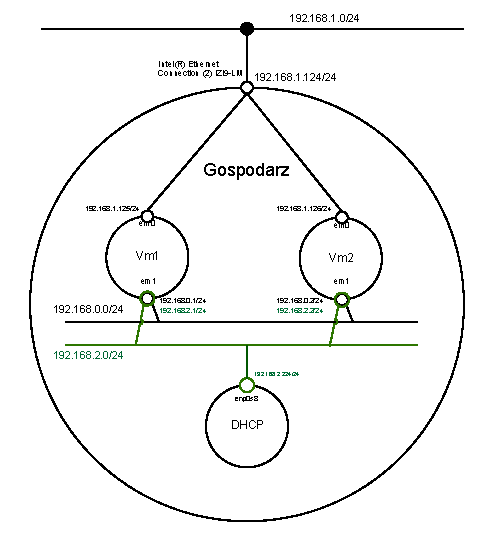
\includegraphics[width=\textwidth]{Projekt_Sieci}
  
  \caption{Schemat budowanej sieci}
  \label{fig:SchematSieci}
\end{figure}

\section{Statyczne adresowanie}
%TODO: Spytać tatę czy może być puste
Ręcznie wybiorę adresy, które przypiszę statycznie interfejsom maszyn.

\subsection{Wybór adresów}
Ponieważ wiem, że będę potrzebował 2 sieci postanowiłem wykorzystać podsieci prywatnej sieci \texttt{192.168.0.0}. W celu ułatwienia obliczeń zdecydowałem, że maska podsieci będzie \textbf{24 bitowa}.

\begin{itemize}
  \item Adres pierwszej sieci -- \texttt{192.168.0.0/24}.
  \item Adres drugiej sieci -- \texttt{192.168.2.0/24}.
\end{itemize}

Maszyna Vm1 otrzyma statyczny adres \texttt{192.168.0.1/24}, a maszyna Vm2 \texttt{192.168.0.2/24}.

\subsection{Ustawienie adresów}
Poleceniem \texttt{ifconfig} sprawdziłem, który interfejs jest podłączony do sieci wewnętrznej. Interfejs \texttt{em0} ma ustawiony adres ip, a \texttt{em1} nie ma. Dzięki temu wiem, że \textbf{em1} jest podłączony do sieci wewnętrznej.

Poleceniem \texttt{ifconfig em1 192.168.0.1/24} nadałem adres. By upewnić się, że polecenie zadziało wywołałem \texttt{ifconfig em1}.

\begin{verbatim}
root@:~ # ifconfig em1
em1: flags=8843<UP,BROADCAST,RUNNING,SIMPLEX,MULTICAST> metric 0 mtu 1500
        options=81009b<RXCSUM,TXCSUM,VLAN_MTU,VLAN_HWTAGGING,VLAN_HWCSUM,VLAN_HWFILTER>
        ether 08:00:27:d1:f2:36
        inet 192.168.0.1 netmask 0xffffff00 broadcast 192.168.0.255
        media: Ethernet autoselect (1000baseT <full-duplex>)
        status: active
        nd6 options=29<PERFORMNUD,IFDISABLED,AUTO_LINKLOCAL>
\end{verbatim}

Postępuje analogicznie na maszynie Vm2 nadając jej adres \texttt{192.168.0.2/24}

\subsection{Test połączenia}
W celu sprawdzenia utworzonej konfiguracji wysłałem ping między maszynami. Będąc zalogowanym na Vm1 wykonałem \texttt{ping -c 3 192.168.0.2}.

\begin{verbatim}
root@:~ # ping -c 3 192.168.0.2
PING 192.168.0.2 (192.168.0.2): 56 data bytes
64 bytes from 192.168.0.2: icmp_seq=0 ttl=64 time=0.597 ms
64 bytes from 192.168.0.2: icmp_seq=1 ttl=64 time=0.749 ms
64 bytes from 192.168.0.2: icmp_seq=2 ttl=64 time=0.849 ms

--- 192.168.0.2 ping statistics ---
3 packets transmitted, 3 packets received, 0.0% packet loss
round-trip min/avg/max/stddev = 0.597/0.732/0.849/0.104 ms
\end{verbatim}

Z wyniku komendy widać, że maszyny są ze sobą połączone i mogą wymieniać informacje.

\section{Dynamiczne adresowanie}
Postanowiłem wykorzystać inną wirtualną maszynę jako serwer DHCP. Wybrałem maszynę z systemem Ubuntu.

\subsection{Konfiguracja serwera}
Maszyna ubuntu ma dwa wirtualne interfejsy fizyczne. Tak jak u Vm1 i Vm2 jeden jest podłączony mostem do gospodarza, a drugi do sieci wewnętrznej \textit{intnet}.

Zainstalowałem serwer DHCP pleceniem \texttt{sudo apt install isc-dhcp-server}. Następnie skonfigurowałem serwer edytując dwa pliki systemowe.

W pliku \texttt{/etc/default/isc-dhcp-server} umieściłem linię \texttt{INTERFACES="enp0s8"}, która wskazuje na jakim interfejsie serwer DHCP ma pracować.

W pliku \texttt{/etc/dhcp/dhcpd.conf} umieściłem konfigurację samego serwera. Zawartość tego pliku wygląda następująco:

\begin{verbatim}
ddns-update-style none;
default-lease-time 600;
max-lease-time 7200;

subnet 192.168.2.0 netmask 255.255.255.0 {
  range 192.168.2.1 192.168.2.253;
}
\end{verbatim}

Definiuje on na jaki czas będą przydzielane adresy oraz z jakie puli będą pochodzić.

Po zakończeniu konfiguracji uruchomiłem serwer poleceniem \texttt{sudo systemctl start isc-dhcp-server.service} oraz \texttt{sudo systemctl enable isc-dhcp-server.service}

\vspace{3mm}
By sprawdzić czy serwer działa wykonałem komendę \texttt{systemctl status isc-dhcp-server.service}.
\begin{verbatim}
  isc-dhcp-server.service - ISC DHCP IPv4 server
   Loaded: loaded (/lib/systemd/system/isc-dhcp-server.service; enabled; vendor preset: enabled)
   Active: active (running) since wto 2019-04-16 18:06:48 CEST; 14min ago
     Docs: man:dhcpd(8)
 Main PID: 3186 (dhcpd)
   CGroup: /system.slice/isc-dhcp-server.service
           3186 dhcpd -user dhcpd -group dhcpd -f -4 -pf /run/dhcp-server/dhcpd.pid -cf /etc/dhcp/dhcpd.conf enp0s8
\end{verbatim}

\subsection{Dynamiczne przydzielenie adresów}
By pozyskać adres od serwera DHCP na maszynach Vm1 i Vm2 uruchomiłem komendę \texttt{dhclient em1}.

\vspace{2mm}
Działanie na maszynie Vm1:
\begin{verbatim}
  # dhclient em1
  DHCPREQUEST on em1 to 255.255.255.255 port 67
  DHCPREQUEST on em1 to 255.255.255.255 port 67
  DHCPDISCOVER on em1 to 255.255.255.255 port 67 interval 7
  DHCPOFFER from 192.168.2.254
  DHCPREQUEST on em1 to 255.255.255.255 port 67
  DHCPACK from 192.168.2.254
  bound to 192.168.2.1 -- renewal in 300 seconds.
\end{verbatim}

Działanie na maszynie Vm2:
\begin{verbatim}
  # dhclient em1
  DHCPDISCOVER on em1 to 255.255.255.255 port 67 interval 6
  DHCPOFFER from 192.168.2.254
  DHCPREQUEST on em1 to 255.255.255.255 port 67
  DHCPACK from 192.168.2.254
  bound to 192.168.2.2 -- renewal in 300 seconds.
\end{verbatim}

Można zaobserwować, że serwer przydzielił dwa pierwsze adresy maszynom.
 
\section{Druga warstwa sieciowa}
Od początku planowałem kładzenie drugiej warstwy sieciowej. Skonfigurowałem serwer DHCP w ten sposób, że przydziela on adresy z drugiej, oddzielnej sieci niż adresy ustawione statycznie. Można to łatwo sprawdzić wywołując \texttt{ifconfig} dla obydwu maszyn.

\paragraph{Vm1:}
\begin{verbatim}
# ifconfig
em0: flags=8843<UP,BROADCAST,RUNNING,SIMPLEX,MULTICAST> metric 0 mtu 1500
        options=81009b<RXCSUM,TXCSUM,VLAN_MTU,VLAN_HWTAGGING,VLAN_HWCSUM,VLAN_HWFILTER>
        ether 08:00:27:a7:2f:18
        inet 192.168.1.121 netmask 0xffffff00 broadcast 192.168.1.255
        media: Ethernet autoselect (1000baseT <full-duplex>)
        status: active
        nd6 options=29<PERFORMNUD,IFDISABLED,AUTO_LINKLOCAL>
em1: flags=8843<UP,BROADCAST,RUNNING,SIMPLEX,MULTICAST> metric 0 mtu 1500
        options=81009b<RXCSUM,TXCSUM,VLAN_MTU,VLAN_HWTAGGING,VLAN_HWCSUM,VLAN_HWFILTER>
        ether 08:00:27:d1:f2:36
        inet 192.168.0.1 netmask 0xffffff00 broadcast 192.168.0.255
        inet 192.168.2.1 netmask 0xffffff00 broadcast 192.168.2.255
        media: Ethernet autoselect (1000baseT <full-duplex>)
        status: active
        nd6 options=29<PERFORMNUD,IFDISABLED,AUTO_LINKLOCAL>
\end{verbatim}

\paragraph{Vm2:}
\begin{verbatim}
# ifconfig
em0: flags=8843<UP,BROADCAST,RUNNING,SIMPLEX,MULTICAST> metric 0 mtu 1500
        options=81009b<RXCSUM,TXCSUM,VLAN_MTU,VLAN_HWTAGGING,VLAN_HWCSUM,VLAN_HWFILTER>
        ether 08:00:27:d2:ad:35
        inet 192.168.1.125 netmask 0xffffff00 broadcast 192.168.1.255
        media: Ethernet autoselect (1000baseT <full-duplex>)
        status: active
        nd6 options=29<PERFORMNUD,IFDISABLED,AUTO_LINKLOCAL>
em1: flags=8843<UP,BROADCAST,RUNNING,SIMPLEX,MULTICAST> metric 0 mtu 1500
        options=81009b<RXCSUM,TXCSUM,VLAN_MTU,VLAN_HWTAGGING,VLAN_HWCSUM,VLAN_HWFILTER>
        ether 08:00:27:9e:5d:3c
        inet 192.168.0.2 netmask 0xffffff00 broadcast 192.168.0.255
        inet 192.168.2.2 netmask 0xffffff00 broadcast 192.168.2.255
        media: Ethernet autoselect (1000baseT <full-duplex>)
        status: active
        nd6 options=29<PERFORMNUD,IFDISABLED,AUTO_LINKLOCAL>
\end{verbatim}

Widać wyraźnie, że interfejsy \texttt{em1} mają przypisane \textbf{dwa} adresy ip z różnych sieci.

\section{Analiza ruchu sieciowego}
W celu zbadania ruchu sieciowego skorzystam z konsolowego narzędzia \texttt{tcpdump}.

\subsection{Badanie ARP}
By przechwycić ruch związany z protokołem ARP uruchomiłem nasłuchiwanie na maszynie Vm1 poleceniem \texttt{tcpdump -i em1 -X arp}.

Maszyna Vm2 ma zapamiętany adres MAC maszyny Vm1 ponieważ wykonywałem pingowanie. Aby to zmienić muszę wyczyścić cashe ARP poleceniem \texttt{arp -d -a}.

Wykonałem polecenie \texttt{ping -c 2 192.168.2.254} na Vm2 by sprowokować użycie ARP.

\paragraph{Wynik działania tcpdump:}
\begin{verbatim}
# tcpdump -i em1 -X arp
tcpdump: verbose output suppressed, use -v or -vv for full protocol decode
listening on em1, link-type EN10MB (Ethernet), capture size 262144 bytes
20:38:26.599494 ARP, Request who-has 192.168.2.254 tell 192.168.2.2, length 46
        0x0000:  0001 0800 0604 0001 0800 279e 5d3c c0a8  ..........'.]<..
        0x0010:  0202 0000 0000 0000 c0a8 02fe 0000 0000  ................
        0x0020:  0000 0000 0000 0000 0000 0000 0000       ..............
^C
1 packet captured
1 packet received by filter
0 packets dropped by kernel
\end{verbatim}

Z przechwyconych informacji można wywnioskować, że maszyna o adresie \texttt{192.168.2.2} pytała o to kto ma adres \texttt{192.168.2.254}.

\subsection{Badanie DHCP}
By przechwycić ruch związany z dynamicznym nadawaniem adresów uruchomiłem nasłuchiwanie na maszynie Vm1 poleceniem \texttt{tcpdump -i em1 port 67 or port 68 -X}.

By móc na nowo pozyskać adres na maszynie Vm2 zatrzymałem działającego klienta DHCP poleceniem \texttt{kill -9 968}. Następnie wywołałem \texttt{dhclient em1}. Zwrócony został następujący komunikat.
\begin{verbatim}
DHCPREQUEST on em1 to 255.255.255.255 port 67
DHCPACK from 192.168.2.254
bound to 192.168.2.2 -- renewal in 300 seconds.
\end{verbatim}

\paragraph{Wynik działania tcpdump:}
\begin{footnotesize}
\begin{verbatim}
tcpdump: verbose output suppressed, use -v or -vv for full protocol decode
listening on em1, link-type EN10MB (Ethernet), capture size 262144 bytes
20:51:51.642745 IP 0.0.0.0.bootpc > 255.255.255.255.bootps: BOOTP/DHCP, Request from 08:00:27:9e:5d:3c
(oui Unknown), length 300
        0x0000:  4510 0148 0000 0000 8011 3996 0000 0000  E..H......9.....
        0x0010:  ffff ffff 0044 0043 0134 f6e2 0101 0600  .....D.C.4......
        0x0020:  524a 342d 0000 0000 0000 0000 0000 0000  RJ4-............
        0x0030:  0000 0000 0000 0000 0800 279e 5d3c 0000  ..........'.]<..
        0x0040:  0000 0000 0000 0000 0000 0000 0000 0000  ................
        0x0050:  0000 0000 0000 0000 0000 0000 0000 0000  ................
        0x0060:  0000 0000 0000 0000 0000 0000 0000 0000  ................
        0x0070:  0000 0000 0000 0000 0000 0000 0000 0000  ................
        0x0080:  0000 0000 0000 0000 0000 0000 0000 0000  ................
        0x0090:  0000 0000 0000 0000 0000 0000 0000 0000  ................
        0x00a0:  0000 0000 0000 0000 0000 0000 0000 0000  ................
        0x00b0:  0000 0000 0000 0000 0000 0000 0000 0000  ................
        0x00c0:  0000 0000 0000 0000 0000 0000 0000 0000  ................
        0x00d0:  0000 0000 0000 0000 0000 0000 0000 0000  ................
        0x00e0:  0000 0000 0000 0000 0000 0000 0000 0000  ................
        0x00f0:  0000 0000 0000 0000 0000 0000 0000 0000  ................
        0x0100:  0000 0000 0000 0000 6382 5363 3501 0332  ........c.Sc5..2
        0x0110:  04c0 a802 023d 0701 0800 279e 5d3c 370a  .....=....'.]<7.
        0x0120:  011c 0279 030f 060c 771a ff00 0000 0000  ...y....w.......
        0x0130:  0000 0000 0000 0000 0000 0000 0000 0000  ................
        0x0140:  0000 0000 0000 0000                      ........
20:51:57.589189 IP 192.168.2.1.bootpc > 192.168.2.254.bootps: BOOTP/DHCP, Request from 08:00:27:d1:f2:36 
(oui Unknown), length 300
        0x0000:  4510 0148 3694 0000 8011 7cb1 c0a8 0201  E..H6.....|.....
        0x0010:  c0a8 02fe 0044 0043 0134 36a6 0101 0600  .....D.C.46.....
        0x0020:  b79b cab7 0000 0000 c0a8 0201 0000 0000  ................
        0x0030:  0000 0000 0000 0000 0800 27d1 f236 0000  ..........'..6..
        0x0040:  0000 0000 0000 0000 0000 0000 0000 0000  ................
        0x0050:  0000 0000 0000 0000 0000 0000 0000 0000  ................
        0x0060:  0000 0000 0000 0000 0000 0000 0000 0000  ................
        0x0070:  0000 0000 0000 0000 0000 0000 0000 0000  ................
        0x0080:  0000 0000 0000 0000 0000 0000 0000 0000  ................
        0x0090:  0000 0000 0000 0000 0000 0000 0000 0000  ................
        0x00a0:  0000 0000 0000 0000 0000 0000 0000 0000  ................
        0x00b0:  0000 0000 0000 0000 0000 0000 0000 0000  ................
        0x00c0:  0000 0000 0000 0000 0000 0000 0000 0000  ................
        0x00d0:  0000 0000 0000 0000 0000 0000 0000 0000  ................
        0x00e0:  0000 0000 0000 0000 0000 0000 0000 0000  ................
        0x00f0:  0000 0000 0000 0000 0000 0000 0000 0000  ................
        0x0100:  0000 0000 0000 0000 6382 5363 3501 033d  ........c.Sc5..=
        0x0110:  0701 0800 27d1 f236 370a 011c 0279 030f  ....'..67....y..
        0x0120:  060c 771a ff00 0000 0000 0000 0000 0000  ..w.............
        0x0130:  0000 0000 0000 0000 0000 0000 0000 0000  ................
        0x0140:  0000 0000 0000 0000                      ........
20:51:57.603089 IP 192.168.2.254.bootps > 192.168.2.1.bootpc: BOOTP/DHCP, Reply, length 300
        0x0000:  4500 0148 f649 4000 4011 bd0b c0a8 02fe  E..H.I@.@.......
        0x0010:  c0a8 0201 0043 0044 0134 8343 0201 0600  .....C.D.4.C....
        0x0020:  b79b cab7 0000 0000 c0a8 0201 c0a8 0201  ................
        0x0030:  c0a8 02fe 0000 0000 0800 27d1 f236 0000  ..........'..6..
        0x0040:  0000 0000 0000 0000 0000 0000 0000 0000  ................
        0x0050:  0000 0000 0000 0000 0000 0000 0000 0000  ................
        0x0060:  0000 0000 0000 0000 0000 0000 0000 0000  ................
        0x0070:  0000 0000 0000 0000 0000 0000 0000 0000  ................
        0x0080:  0000 0000 0000 0000 0000 0000 0000 0000  ................
        0x0090:  0000 0000 0000 0000 0000 0000 0000 0000  ................
        0x00a0:  0000 0000 0000 0000 0000 0000 0000 0000  ................
        0x00b0:  0000 0000 0000 0000 0000 0000 0000 0000  ................
        0x00c0:  0000 0000 0000 0000 0000 0000 0000 0000  ................
        0x00d0:  0000 0000 0000 0000 0000 0000 0000 0000  ................
        0x00e0:  0000 0000 0000 0000 0000 0000 0000 0000  ................
        0x00f0:  0000 0000 0000 0000 0000 0000 0000 0000  ................
        0x0100:  0000 0000 0000 0000 6382 5363 3501 0536  ........c.Sc5..6
        0x0110:  04c0 a802 fe33 0400 0002 5801 04ff ffff  .....3....X.....
        0x0120:  00ff 0000 0000 0000 0000 0000 0000 0000  ................
        0x0130:  0000 0000 0000 0000 0000 0000 0000 0000  ................
        0x0140:  0000 0000 0000 0000                      ........
^C
3 packets captured
7 packets received by filter
0 packets dropped by kernel
\end{verbatim}
\end{footnotesize}

\end{document}
